%----------------------------------------------------------------------------------------
%	PACKAGES AND OTHER DOCUMENT CONFIGURATIONS
%----------------------------------------------------------------------------------------

\documentclass[11pt]{article}

%%%%%%%%%%%%%%%%%%%%%%%%%%%%%%%%%%%%%%%%%
% Lachaise Assignment
% Structure Specification File
% Version 1.0 (26/6/2018)
%
% This template originates from:
% http://www.LaTeXTemplates.com
%
% Authors:
% Marion Lachaise & François Févotte
% Vel (vel@LaTeXTemplates.com)
%
% License:
% CC BY-NC-SA 3.0 (http://creativecommons.org/licenses/by-nc-sa/3.0/)
% 
%%%%%%%%%%%%%%%%%%%%%%%%%%%%%%%%%%%%%%%%%

%----------------------------------------------------------------------------------------
%	PACKAGES AND OTHER DOCUMENT CONFIGURATIONS
%----------------------------------------------------------------------------------------

\usepackage{amsmath,amsfonts,stmaryrd,amssymb} % Math packages

\usepackage{enumerate} % Custom item numbers for enumerations

\usepackage[ruled]{algorithm2e} % Algorithms

\usepackage[framemethod=tikz]{mdframed} % Allows defining custom boxed/framed environments

\usepackage{listings} % File listings, with syntax highlighting
\lstset{
	basicstyle=\ttfamily, % Typeset listings in monospace font
}
\usepackage{booktabs}
\usepackage[sort&compress,numbers]{natbib}
%----------------------------------------------------------------------------------------
%	DOCUMENT MARGINS
%----------------------------------------------------------------------------------------

\usepackage{geometry} % Required for adjusting page dimensions and margins

\geometry{
	paper=a4paper, % Paper size, change to letterpaper for US letter size
	top=2.5cm, % Top margin
	bottom=3cm, % Bottom margin
	left=2.5cm, % Left margin
	right=2.5cm, % Right margin
	headheight=14pt, % Header height
	footskip=1.5cm, % Space from the bottom margin to the baseline of the footer
	headsep=1.2cm, % Space from the top margin to the baseline of the header
	%showframe, % Uncomment to show how the type block is set on the page
}

%----------------------------------------------------------------------------------------
%	FONTS
%----------------------------------------------------------------------------------------

\usepackage[utf8]{inputenc} % Required for inputting international characters
\usepackage[T1]{fontenc} % Output font encoding for international characters

\usepackage{XCharter} % Use the XCharter fonts

%----------------------------------------------------------------------------------------
%	COMMAND LINE ENVIRONMENT
%----------------------------------------------------------------------------------------

% Usage:
% \begin{commandline}
%	\begin{verbatim}
%		$ ls
%		
%		Applications	Desktop	...
%	\end{verbatim}
% \end{commandline}

\mdfdefinestyle{commandline}{
	leftmargin=10pt,
	rightmargin=10pt,
	innerleftmargin=15pt,
	middlelinecolor=black!50!white,
	middlelinewidth=2pt,
	frametitlerule=false,
	backgroundcolor=black!5!white,
	frametitle={Command Line},
	frametitlefont={\normalfont\sffamily\color{white}\hspace{-1em}},
	frametitlebackgroundcolor=black!50!white,
	nobreak,
}

% Define a custom environment for command-line snapshots
\newenvironment{commandline}{
	\medskip
	\begin{mdframed}[style=commandline]
}{
	\end{mdframed}
	\medskip
}

%----------------------------------------------------------------------------------------
%	FILE CONTENTS ENVIRONMENT
%----------------------------------------------------------------------------------------

% Usage:
% \begin{file}[optional filename, defaults to "File"]
%	File contents, for example, with a listings environment
% \end{file}

\mdfdefinestyle{file}{
	innertopmargin=1.6\baselineskip,
	innerbottommargin=0.8\baselineskip,
	topline=false, bottomline=false,
	leftline=false, rightline=false,
	leftmargin=2cm,
	rightmargin=2cm,
	singleextra={%
		\draw[fill=black!10!white](P)++(0,-1.2em)rectangle(P-|O);
		\node[anchor=north west]
		at(P-|O){\ttfamily\mdfilename};
		%
		\def\l{3em}
		\draw(O-|P)++(-\l,0)--++(\l,\l)--(P)--(P-|O)--(O)--cycle;
		\draw(O-|P)++(-\l,0)--++(0,\l)--++(\l,0);
	},
	nobreak,
}

% Define a custom environment for file contents
\newenvironment{file}[1][File]{ % Set the default filename to "File"
	\medskip
	\newcommand{\mdfilename}{#1}
	\begin{mdframed}[style=file]
}{
	\end{mdframed}
	\medskip
}

%----------------------------------------------------------------------------------------
%	NUMBERED QUESTIONS ENVIRONMENT
%----------------------------------------------------------------------------------------

% Usage:
% \begin{question}[optional title]
%	Question contents
% \end{question}

\mdfdefinestyle{question}{
	innertopmargin=1.2\baselineskip,
	innerbottommargin=0.8\baselineskip,
	roundcorner=5pt,
	nobreak,
	singleextra={%
		\draw(P-|O)node[xshift=1em,anchor=west,fill=white,draw,rounded corners=5pt]{%
		Question \theQuestion\questionTitle};
	},
}

\newcounter{Question} % Stores the current question number that gets iterated with each new question

% Define a custom environment for numbered questions
\newenvironment{question}[1][\unskip]{
	\bigskip
	\stepcounter{Question}
	\newcommand{\questionTitle}{~#1}
	\begin{mdframed}[style=question]
}{
	\end{mdframed}
	\medskip
}

%----------------------------------------------------------------------------------------
%	NUMBERED MEMBER ENVIRONMENTS
%----------------------------------------------------------------------------------------

% Usage:
% \begin{member}[optional title]
%	member contents
% \end{member}

\mdfdefinestyle{member}{
	innertopmargin=1.2\baselineskip,
	innerbottommargin=0.8\baselineskip,
	roundcorner=5pt,
	nobreak,
	singleextra={%
		\draw(P-|O)node[xshift=1em,anchor=west,fill=white,draw,rounded corners=5pt]{%
		Group Member \theMember\memberTitle};
	},
}

\newcounter{Member} % Stores the current question number that gets iterated with each new question

% Define a custom environment for numbered questions
\newenvironment{member}[1][\unskip]{
	\bigskip
	\stepcounter{Member}
	\newcommand{\memberTitle}{~#1}
	\begin{mdframed}[style=member]
}{
	\end{mdframed}
	\medskip
}
%----------------------------------------------------------------------------------------
%	WARNING TEXT ENVIRONMENT
%----------------------------------------------------------------------------------------

% Usage:
% \begin{warn}[optional title, defaults to "Warning:"]
%	Contents
% \end{warn}

\mdfdefinestyle{warning}{
	topline=false, bottomline=false,
	leftline=false, rightline=false,
	nobreak,
	singleextra={%
		\draw(P-|O)++(-0.5em,0)node(tmp1){};
		\draw(P-|O)++(0.5em,0)node(tmp2){};
		\fill[black,rotate around={45:(P-|O)}](tmp1)rectangle(tmp2);
		\node at(P-|O){\color{white}\scriptsize\bf !};
		\draw[very thick](P-|O)++(0,-1em)--(O);%--(O-|P);
	}
}

% Define a custom environment for warning text
\newenvironment{warn}[1][Warning:]{ % Set the default warning to "Warning:"
	\medskip
	\begin{mdframed}[style=warning]
		\noindent{\textbf{#1}}
}{
	\end{mdframed}
}

%----------------------------------------------------------------------------------------
%	INFORMATION ENVIRONMENT
%----------------------------------------------------------------------------------------

% Usage:
% \begin{info}[optional title, defaults to "Info:"]
% 	contents
% 	\end{info}

\mdfdefinestyle{info}{%
	topline=false, bottomline=false,
	leftline=false, rightline=false,
	nobreak,
	singleextra={%
		\fill[black](P-|O)circle[radius=0.4em];
		\node at(P-|O){\color{white}\scriptsize\bf i};
		\draw[very thick](P-|O)++(0,-0.8em)--(O);%--(O-|P);
	}
}

% Define a custom environment for information
\newenvironment{info}[1][Info:]{ % Set the default title to "Info:"
	\medskip
	\begin{mdframed}[style=info]
		\noindent{\textbf{#1}}
}{
	\end{mdframed}
}


\bibliographystyle{unsrt3author}
 % Include the file specifying the document structure and custom commands

%----------------------------------------------------------------------------------------
%	Proposal INFORMATION
%----------------------------------------------------------------------------------------

\title{COVID-19 Classification Based on Cough Sound} % Title of the assignment

\author{COMP5331 Course Project Group 2} % Author name and email address

\date{The Hong Kong University of Science and Technology --- \today} % University, school and/or department name(s) and a date

%----------------------------------------------------------------------------------------

\begin{document}

\maketitle % Print the title

%----------------------------------------------------------------------------------------
%	Basic Information
%----------------------------------------------------------------------------------------

\section{Basic Information}
\subsection{Project information}
Our project is COVID-19 classification based on cough sound. Table \ref{tab1} describes other project and group information.
\begin{table}[!htbp]
	\caption{Project and group information} \centering
	\label{tab1}
	\begin{tabular}{ccc}
	\toprule[1.5pt]
	Project topic & Project type & Group number \\
    \midrule[1pt]
    Classification & Implementation & 2 \\
	\bottomrule[1.5pt]
	\end{tabular}
\end{table}

\subsection{Group Information}
Group 2 consists of six group members: CHAO Chung-chi, LI Jiabao, MO Zongchao, TANG Jihong,
WANG Yubo, YANG Lingyun. The detailed information about these members is as
follows.

\begin{member}
	\begin{enumerate}[(a)]
		\item Student ID: 20562119
		\item Student Name: Chung-chi CHAO
		\item FYP supervisor: Prof. Shing-Chi CHEUNG
		\item FYP topic and explanation: \\
		My FYP topic is deep testing of DNN systems. We are aiming to provide a set of detection criteria to uncover faults in DNN systems especially in the data aspect. The work will mostly be focused on designing and implementing rules to detect and categorize potential data faults given an input dataset, which is not related to this group project.
		\item Declaration statement: \\
		I declare that this project is done solely within the course but not other scopes.
	\end{enumerate}
\end{member}

\begin{member}
	\begin{enumerate}[(a)]
		\item Student ID: 20718615
		\item Student Name: Jiabao LI
		\item Research supervisor: Prof. Jiguang WANG
		\item Research topic and explanation: \\
		My research topic is to uncover the evolution process within biology, mostly in cancer genomics and radiomics. I am working on the simulation and the calculation of the brain tumor by machine learning, which is unrelated to the group project.
		\item Declaration statement: \\
		I declare that this project is done solely within the course but not other scopes.
	\end{enumerate}
\end{member}

\begin{member}
	\begin{enumerate}[(a)]
		\item Student ID: 20755950
		\item Student Name: Zongchao MO
		\item FYP supervisor: Prof. Jiguang WANG
		\item FYP topic and explanation: \\
		Computational biology. My research mainly focuses on computational biology. We analyze cancer genome sequencing data to identify both germline and somatic genome alteration contributing to tumorigenesis and development. And we use computational methods to investigate the dynamic expression change during cancer treatment.
		\item Declaration statement: \\
		I declare that this project is done solely within the course but not other scopes.
	\end{enumerate}
\end{member}

\begin{member}
	\begin{enumerate}[(a)]
		\item Student ID: 20815724
		\item Student Name: Jihong TANG
		\item Research supervisor: Prof. Jiguang WANG
		\item Research topic and explanation: \\
		As a first year PhD student, my research topic has not been focused. But my supervisor and my lab have focused on brain tumor related computational  methods development and data analysis. Therefore, my future research work will be related to the brain tumor with a high probability, which is not related with the course project.
		\item Declaration statement: \\
		I declare that this project is done solely within the course but not other scopes.
	\end{enumerate}
\end{member}

\begin{member}
	\begin{enumerate}[(a)]
		\item Student ID: 20840755
		\item Student Name: Yubo WANG
		\item Research supervisor: Prof. Lei CHEN
		\item Research topic and explanation: \\
		Knowledge Extraction. The knowledge extraction procedure is a way that we could obtain information and data from sources like web pages or html files. Because the data contained in the data sources are usually not formatted, therefore we develop various methods or algorithms to extract them. Hence my research topic is nothing related to the classification work.
		\item Declaration statement: \\
		I declare that this project is done solely within the course but not other scopes.
	\end{enumerate}
\end{member}

\begin{member}
	\begin{enumerate}[(a)]
		\item Student ID: 20715584
		\item Student Name: Lingyun YANG
		\item Research supervisor: Prof. Wei WANG
		\item Research topic and explanation: \\
		My research interests include machine learning for systems, cloud computing and resource management for large-scale clusters. Currently, I am working on the research mainly about resource management for large-scale gpu clusters. In this project, our group chooses a topic on COVID-19 cough classification, which is different from my own research.
		\item Declaration statement: \\
		I declare that this project is done solely within the course but not other scopes.

	\end{enumerate}
\end{member}

%----------------------------------------------------------------------------------------
%	Project description
%----------------------------------------------------------------------------------------

\section{Introduction}

Since December 2019, the coronavirus disease 2019 (COVID-19) has been the health hotspot worldwide. Caused by severe acute respiratory syndrome coronavirus 2 (SARS-CoV-2), COVID-19 has been highly transmissible and spread fast around the whole world. Since 2021, variants of the virus have emerged and become dominant in many countries, with the Delta, Alpha and Beta variants being the most virulent. COVID-19 has confirmed cases exceeding 228 million world-wide \cite{wiki2021covid19}. Different variants of the virus gave them the ability to survive under the pressure of vaccines. Despite the global vaccination, the COVID-19 has caused more than  4.68 million deaths, making it one of the deadliest pandemics in history.

The diagnosis of COVID-19 is made primarily by direct detection of SARS-CoV-2 RNA by nucleic acid amplification tests (NAATs). In addition to the direct detection method, multiple methods focusing on the fast, easily-accessible and possible contactless diagnosis of COVID-19 have been developed by the research and industry community. Among which, the usage of cough sound collected from smartphone apps, trained with machine learning or deep learning models, for detecting and classifying COVID-19 has become popular recently \cite{xue2021exploring}. The cough sound based diagnosis method shows its advantage in different areas. Firstly, it may decrease the demands for facilities and resources compared to NAAT methods, such as medical supplies and experienced workers. Secondly, it may decrease the transmisible risk for its contactless data collection procedure.

However, more data preprocessing and modeling development work needed to be done to increase the accuracy of such methods. Therefore, we propose to put our focus on the diagnosis method based on cough sound in this course project. We aim to implement the most popular classification models in related papers, and give our own evaluations based on their performances.

\section{Related Work}

Various machine learning and deep learning models have been explored on the task of COVID-19 sound classification. There are two main groups of methods approaching the classification problem, which is Convolutional Neural Network (CNN) based and Recurrent Neural Network (RNN) based. Traditionally, ResNet, VGG and other prominent deep learning models are used for image classification task. And they have also been adopted in COVID-19 lung CT images classification task \cite{sitaula2021attention,rahimzadeh2020modified}. There have also been recent work applying CNN structures to proform audio classification by transforming the audio dato to Mel Frequency Cepstral Coefficients (MFCC). Classification on COVID-19 cough sounds using ResNet and VGG based CNNs have also been explored by \cite{schuller2020detecting,brown2020exploring}. VGGish has also been explored to extract audio features in COVID-19 cough sound. On the other hand, Variational Autoencoder has also been applied to COVID-19 image classification task to encode the data \cite{mansour2021unsupervised} and general sound classification tasks \cite{teh2021open}.

The group of methods adopting RNNs including model variations as Long Short Term Memory (LSTM) and Gated Recurrent Units (GRU) takes advantage of the models’ ability to process temporal sequence data on COVID-19 cough sound. Recent research have explored LSTM models to perform COVID-19 cough sound classification task \cite{hassan2020covid,pahar2021covid}. While there has been less work focusing on the usage of GRU on COVID-19 sound classification task only but more on audio scene classification \cite{phan2017audio}. 

\section{Dataset}

\subsection{Data Acquisition \& Analysis}

We used the data from Project Coswara to finish our project based on our proposal. The Project Coswara by Indian Institute of Science (IISc) Bangalore is an attempt to build a diagnostic tool for Covid-19 based on respiratory, cough and speech sounds. We downloaded all the data from their Github Homepage \cite{coswara}, and found that the data amount is large and contained many interesting features including both continuous and discrete variables.

We use several data analysis and visualization methods to get familiar with the raw data and try to determine the final labeling methods that will be shared during all the following classification modeling procedures. Feature table for the coswara dataset was extracted directly from their Github Homepage and analysised using the R programming language. The data analysis could be divided into two parts: descriptive analysis and correlation analysis.

For the descriptive analysis part, we visualized several important and well-organized features. First of all, we are curious about the covid status, which could be the potential labeling variable.

\begin{figure}[!htbp]{}
    \centering
    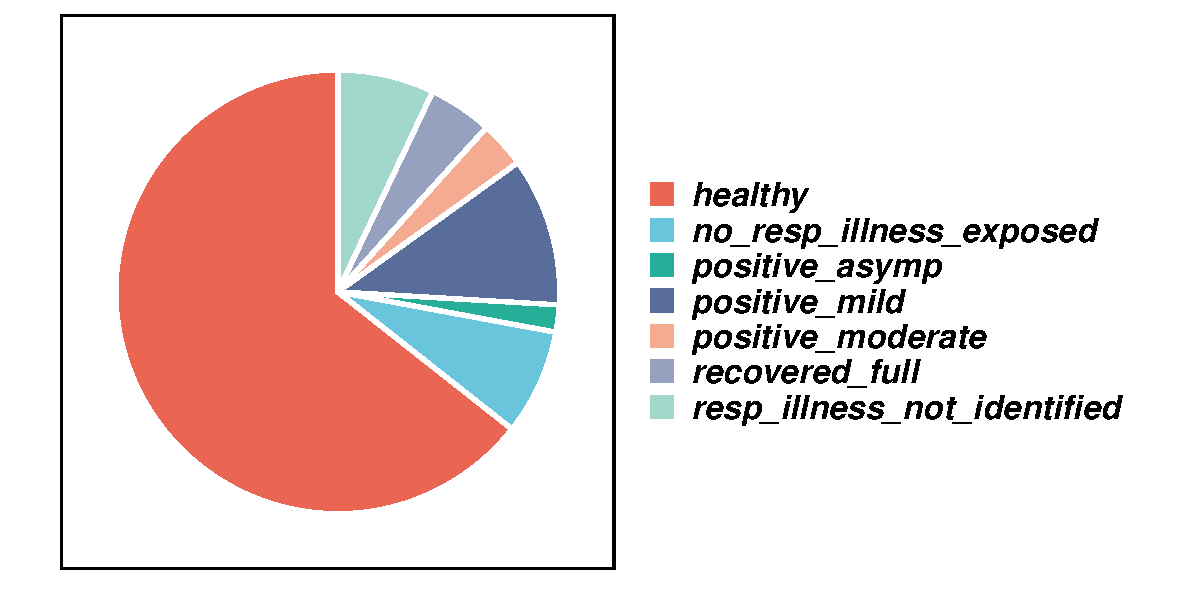
\includegraphics[width=.8\textwidth]{./imgs/pie_covid_status.pdf} % requires the graphicx package
    \caption{Distribution of covid status}
    \label{fig:pie_covid_status}
\end{figure}

As shown in Figure \ref{fig:pie_covid_status}, there are seven different covid status totally, and the pattern frequency ranges from 1.9\% (positive\_asymp) to 64.4\% (healthy). Such distribution is very imbalanced and is not suitable to act as the labeling pattern. Therefore, we tried to relabel all the subjects into two categories: healthy ones and all the others as unhealthy ones. Based on such labeling criteria, the distribution of labeling patterns becomes more balanced. Finally, among all the 2128 subjects, 1370 (64.4\%) are labeled healthy and 758 (35.6\%) are labeled unhealthy (Figure \ref{fig:pie_label}).

\begin{figure}[htbp]{}
	\centering
    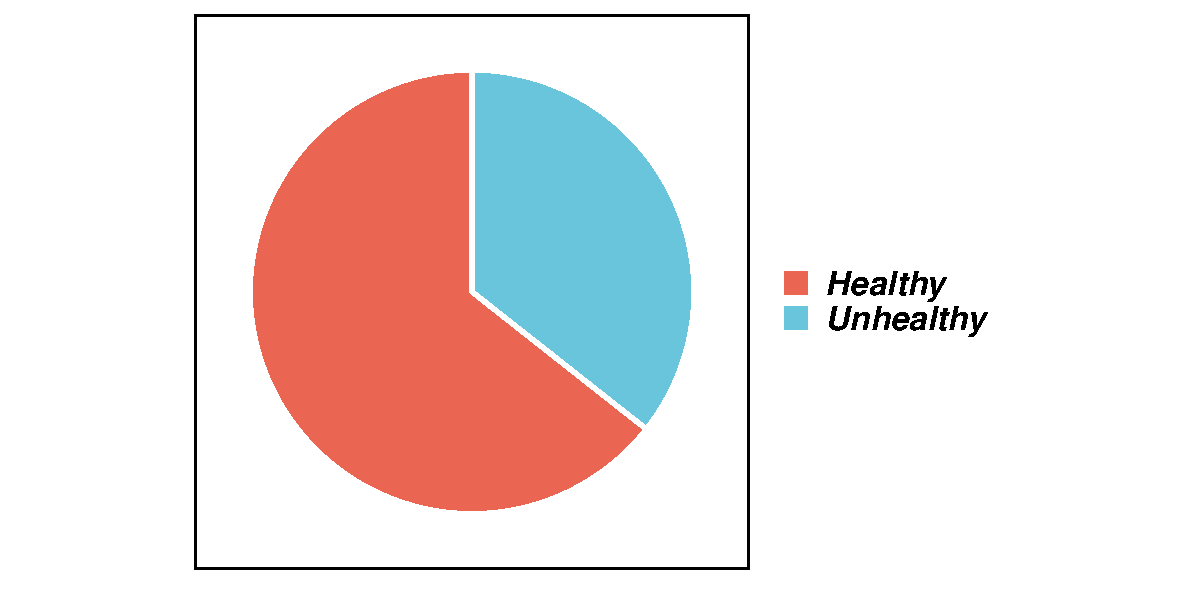
\includegraphics[width=.8\textwidth]{./imgs/pie_label.pdf} % requires the graphicx package
    \caption{Distribution of label}
    \label{fig:pie_label}
\end{figure}

In addition to the labeling pattern, we also looked at the distribution of the gender pattern among all the subjects. (Figure \ref{fig:pie_gender})

\begin{figure}[htbp]{}
	\centering
    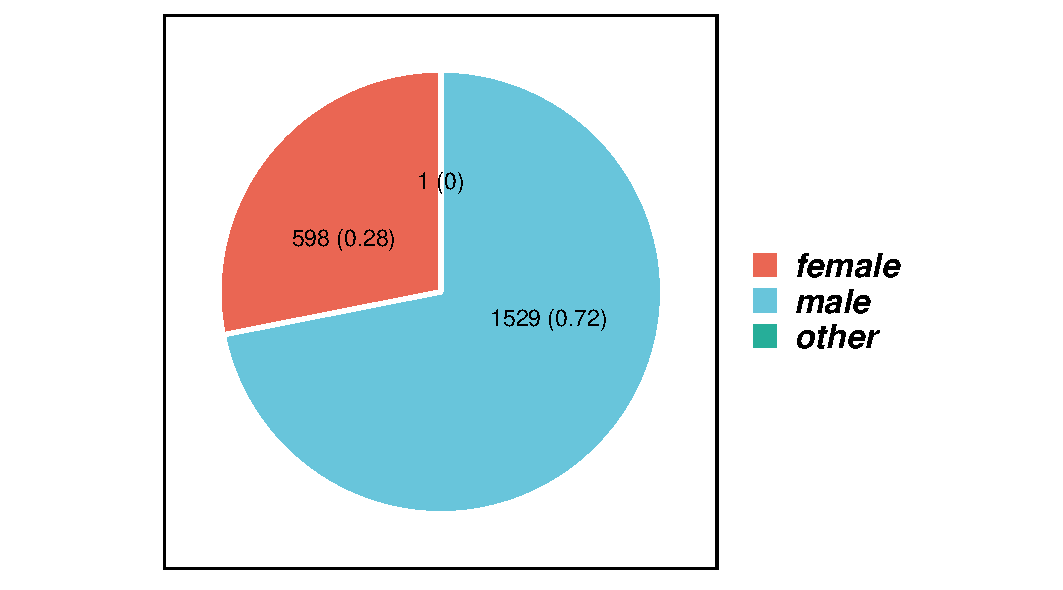
\includegraphics[width=.8\textwidth]{./imgs/pie_gender.pdf} % requires the graphicx package
    \caption{Distribution of gender}
    \label{fig:pie_gender}
\end{figure}

The age is the only one continuous pattern among all the patterns, therefore, we proposed to verify the necessity of relabeling based on the age pattern. Based on our analysis of the distribution for different labeling methods (Figure \ref{fig:distri_label_age}, Figure \ref{fig:distri_status_age}). The relabeling to binary patterns as healthy and unhealthy definitely have more obvious features and deserve future usage.

\begin{figure}[htbp]{}
	\centering
    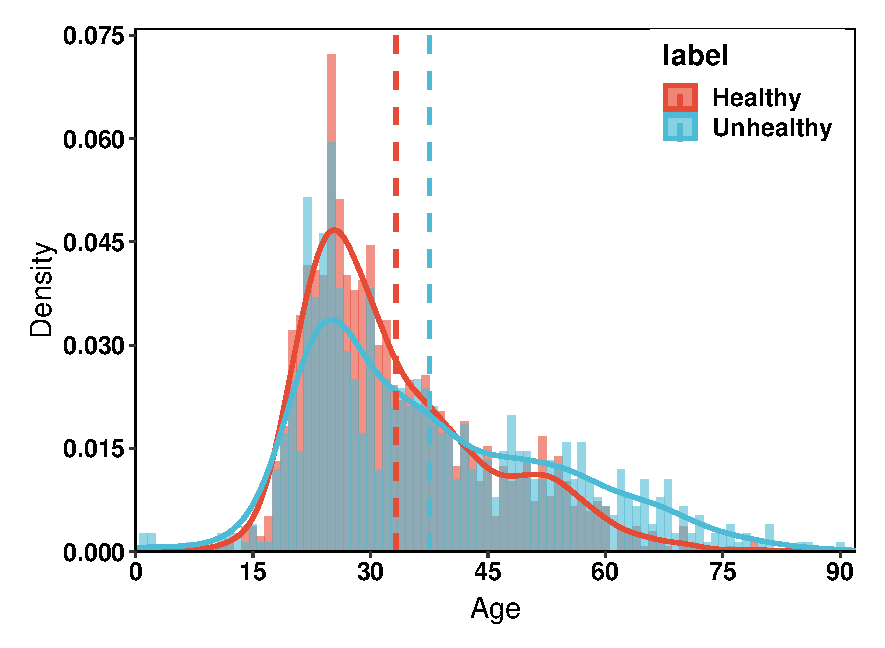
\includegraphics[width=.8\textwidth]{./imgs/distri_label_age.pdf} % requires the graphicx package
    \caption{Distribution of age based on binary labeling system}
    \label{fig:distri_label_age}
\end{figure}

\begin{figure}[htbp]{}
	\centering
    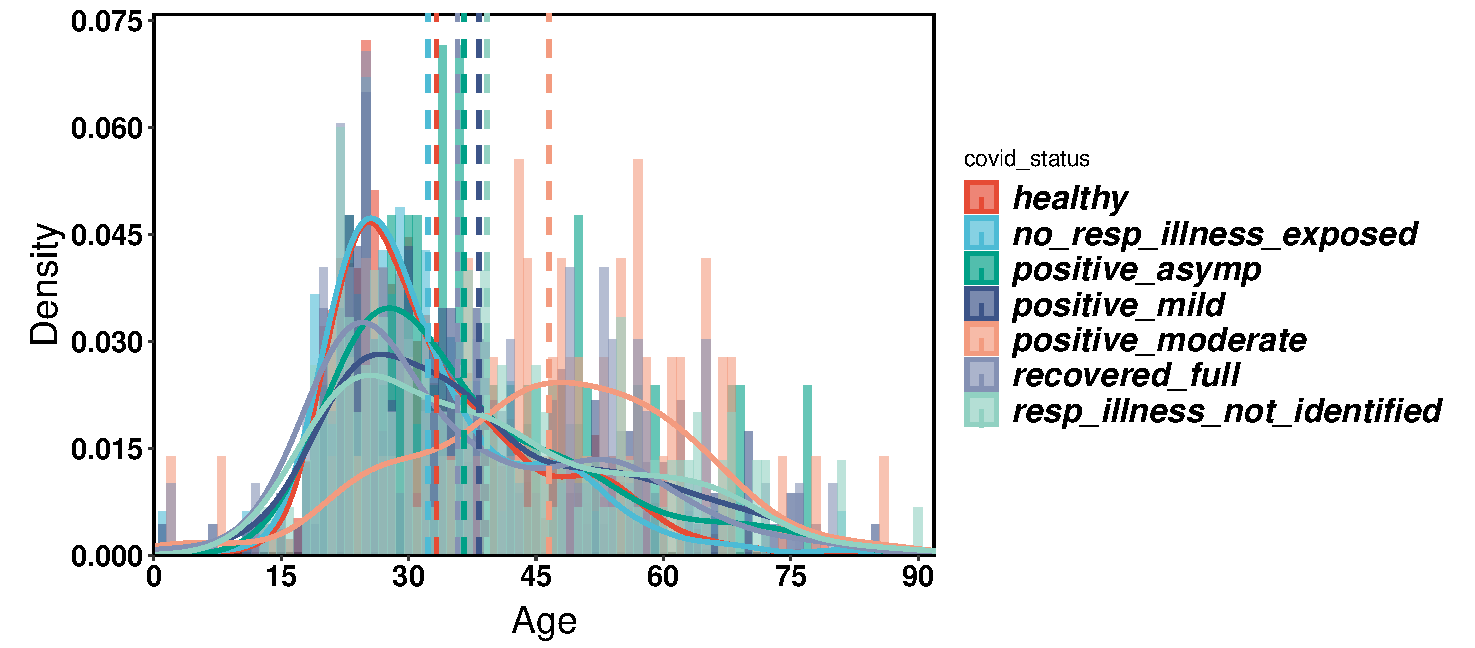
\includegraphics[width=.8\textwidth]{./imgs/distri_status_age.pdf} % requires the graphicx package
    \caption{Distribution of age based on multiclass labeling system}
    \label{fig:distri_status_age}
\end{figure}

For the correlation part, we used four parameters to compare the correlation between the patterns and the different label system. The first one is the pearson’s X-square coefficient, the larger the number, the weaker the correlation between two variables.  The second one is the Contingency coefficient C, which is the normalized version of pearson’s X-square coefficient and shares the same trendency. The third one is the Cramer’s V, for a $k \times l$ contingency table, $n(min(k,l)-1)$ is the maximal value of the $\chi^2$ statistic, dividing $\chi^2$ by the maximal value leads to a scaled version with maximal value 1. This idea is used by Cramer’s V and shares the similar trendency. The fourth is the uncertainty coefficient (also called entropy coefficient or Thiel’s U), which is a measure of nominal association. It is based on the concept of information entropy. Similarly, the smaller the U, the stronger the correlation between two variables. Based on our correlation analysis result, almost all the features show a stronger relationship to the binary labeling system for all of the coefficients. That is one evidence for our choice of the binary labeling system.

\begin{table}
	\centering
	\begin{tabular}[!htbp]{|c|c|}
	\hline
	Pattern & Meanings\\
	\hline
	asthma & Asthma (True/False)\\
	\hline
	cough & Cough (True/False)\\
	\hline
	smoker & Smoker (True/False)\\
	\hline
	ep & Proficient in English (y/n)\\
	\hline
	ht & Hypertension  (True/False)\\
	\hline
	ihd & Ischemic Heart Disease (True/False)\\
	\hline
	cold & Cold (True/False)\\
	\hline
	\end{tabular}
	\caption{Patterns and their meanings}
\end{table}

\begin{figure}[htbp]{}
	\centering
    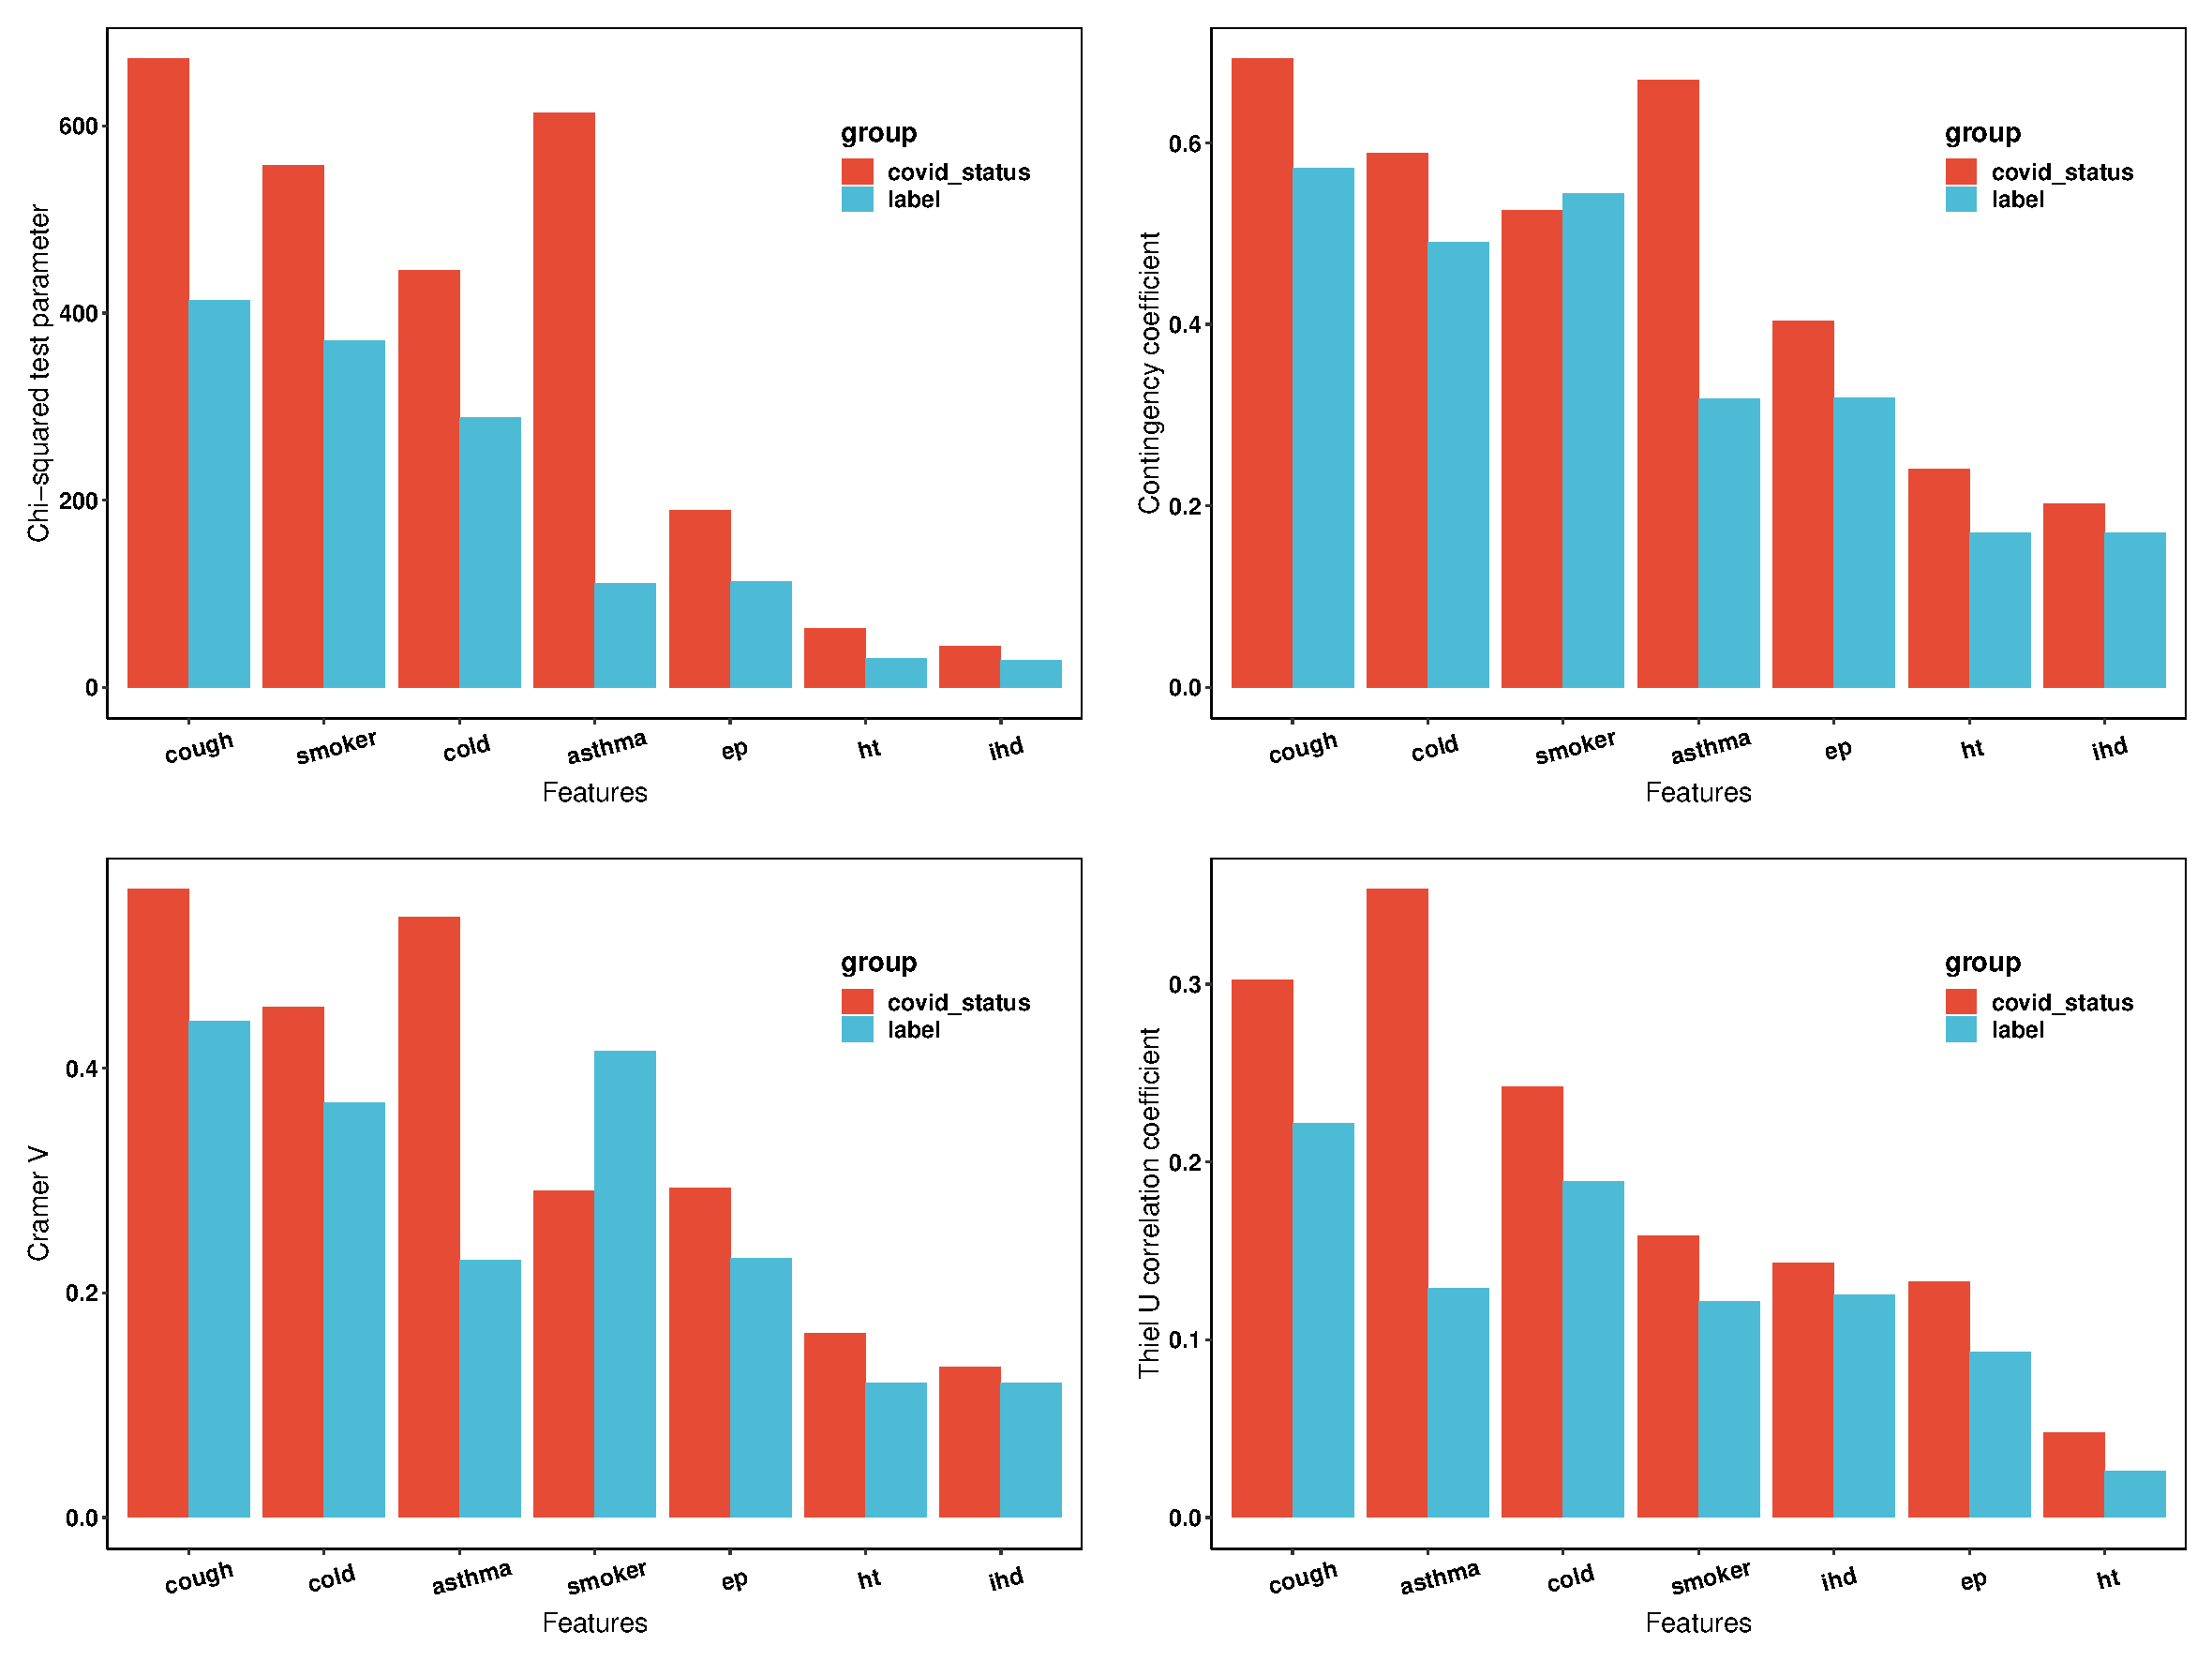
\includegraphics[width=1.0\textwidth]{./imgs/cor_total.pdf} % requires the graphicx package
    \caption{Correlation for all coefficients}
    \label{fig:cor_total}
\end{figure}

\subsection{Data Pre-processing}

After we acquired the coswara dataset, we use the methods in \cite{xue2021exploring} to pre-process the audio into the clean features by the universal methods of the digital signal processing. In the coswara dataset, there are totally 2130 patient IDs by the time of 20210914 and there are 8-9 audio files in each patient's folders. Some of the patients have all the audio information such as the audio of breathing-shallow, the audio of breathing-deep, the audio of cough-shallow, the audio of cough-heavy, the audio of counting normal, the audio of counting fast, the audio of vowel-a, the audio of vowel-e and the audio of vowel-e, in total nine audio files. However, some patients may not have all the audio files or some of the audio files are defected. Therefore, we pre-process the coswara dataset in several steps as follows:

\begin{enumerate}
	\item Remove the patients who don’t have all the audio files.
	\item Remove the patients whose audio files are available or there are some errors on the audio files.
	\item Extract the MFCC features from the audio files.
\end{enumerate}

As shown in Figure \ref{fig:clean_unavailable_audio}, even though some patients have all the audio files, the size of the audio files is too small (just 44B) and we are also removing the patients (totally 65 patients) on this occasion. After removing the patients in step one and step two, we remove another 65 patients whose audio files have errors, and there are totally 2063 patients after the data cleaning.
Then we implement the feature extraction steps according to the guidance of the article \cite{xue2021exploring}. As is mentioned in the article we would like to implement, the Mel Frequency Cepstral Coefficients (MFCC) based on fast Fourier transform (FFT) is one of the methods widely used in audio analysis. We use the python speech features library \cite{pyspeech} to get the MFCC feature matrix in the following steps. First we collected all the audio files for the patients, then we used the read() function in scipy.io.wavfile module to read the audio files in wav format into the sample rate as well as the wav matrix in numpy array format. Then we use the logfbank function to get the log-compressed mel-filter banks with size of FFT equal to 4800. In this case, we will get the extracted MFCC matrix for all the audios from the patients. To implement the model by the article, we set the number of the filters in the filterbank as 26 default instead of 64 initialization, which will help us get more compressed MFCC features and speed up the training processes in our own laptops.

\begin{figure}[htbp]{}
	\centering
    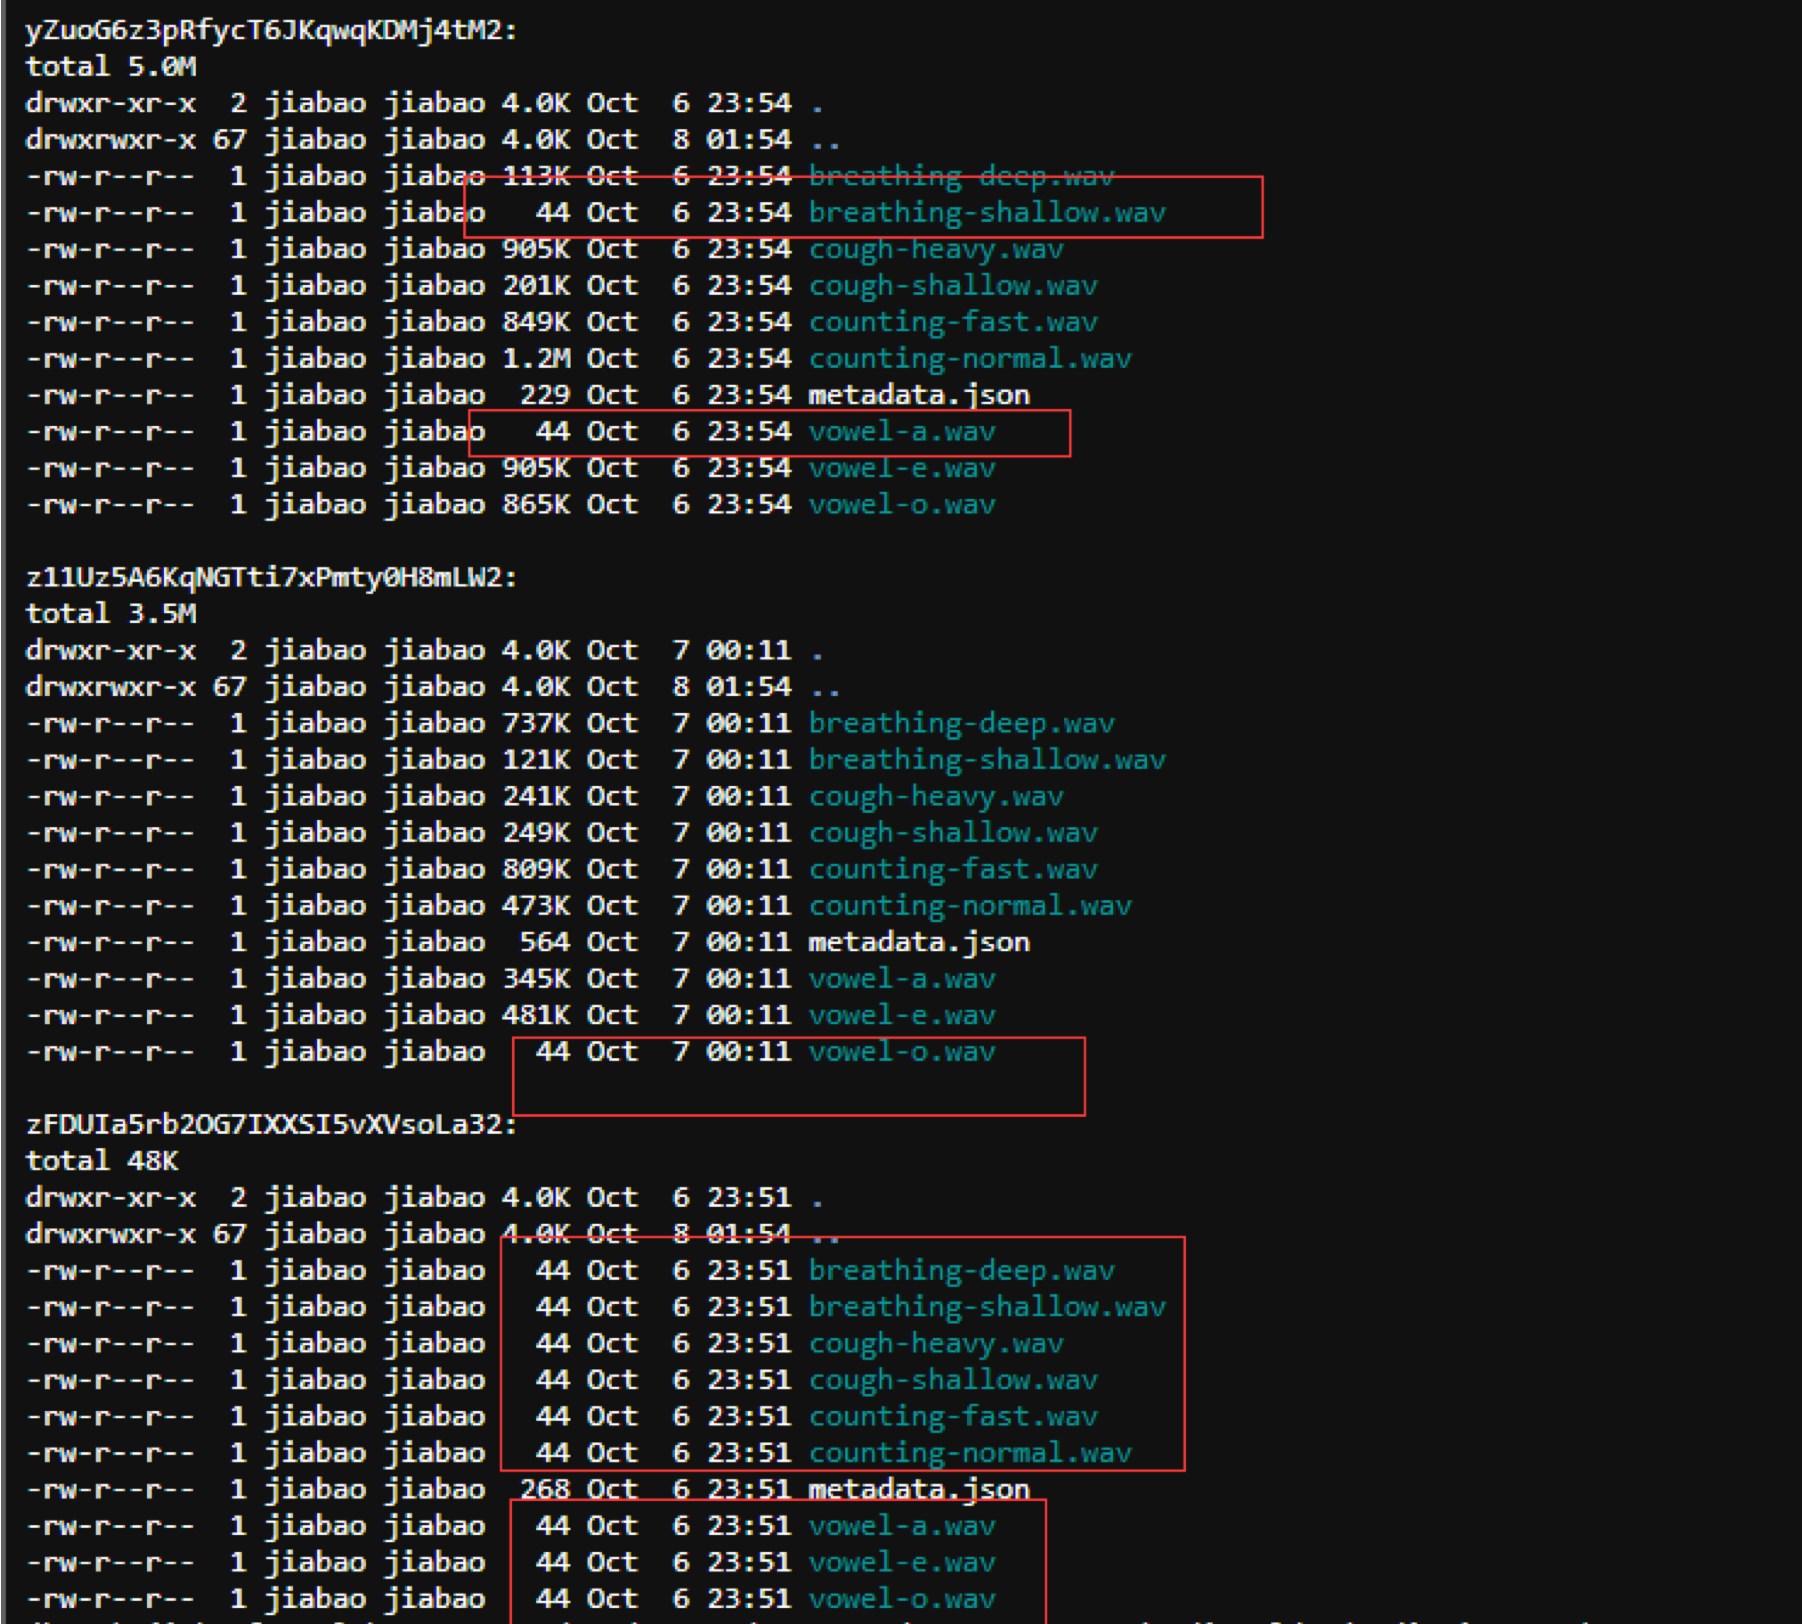
\includegraphics[width=0.8\textwidth]{./imgs/mfccFig1-new.png} % requires the graphicx package
    \caption{Clean the unavailable audio files}
    \label{fig:clean_unavailable_audio}
\end{figure}

Figures \ref{fig:audio_matrix_mfcc} show the example results before and after the MFCC extraction in the pre-process steps. The left one is the wav array for the audio which is extracted by the scipy package and the right one is the log-compressed mel-filter banks acquired by the python speech features library package we used. By comparing the input audios and the output MFCC matrix, there are 26 features extracted for each bank, and the number of the bank is due to the length of the original audio files.
To sum up, in this step, data cleaning and preprocessing are implemented. We removed the patients who don’t have all the audio files or have some damaged audio files. Then we extract the MFCC matrix for all the audio files in all the patients. In the next step of the models, the pre-processed data as well as the labels will be regarded as the input for the models and perform the classification.

\begin{figure}[htbp]{}
	\centering
    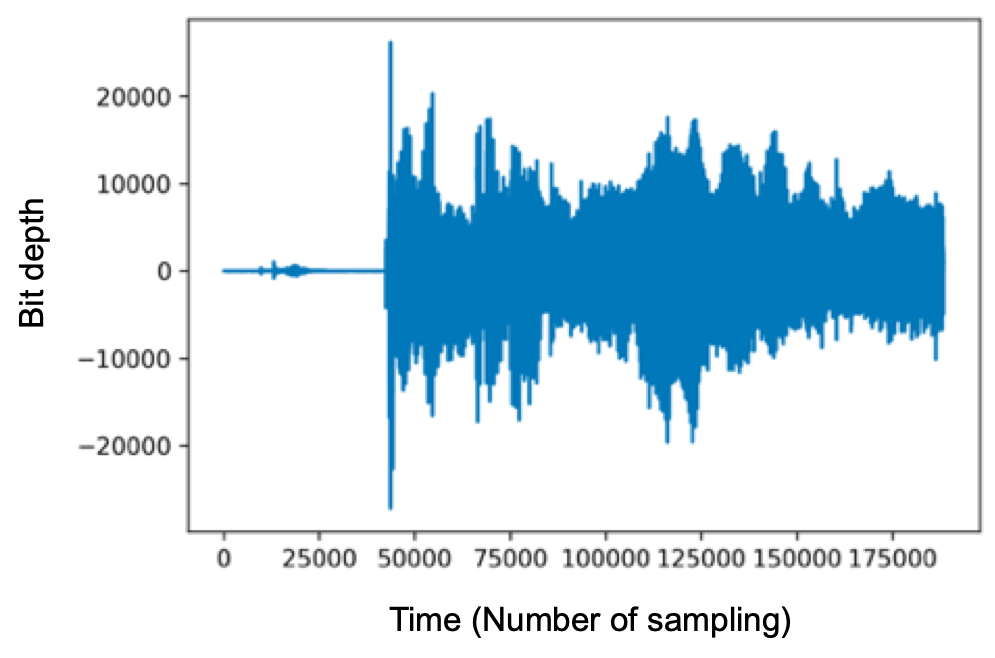
\includegraphics[width=0.4\textwidth]{./imgs/mfccFig2-new.png} % requires the graphicx package
    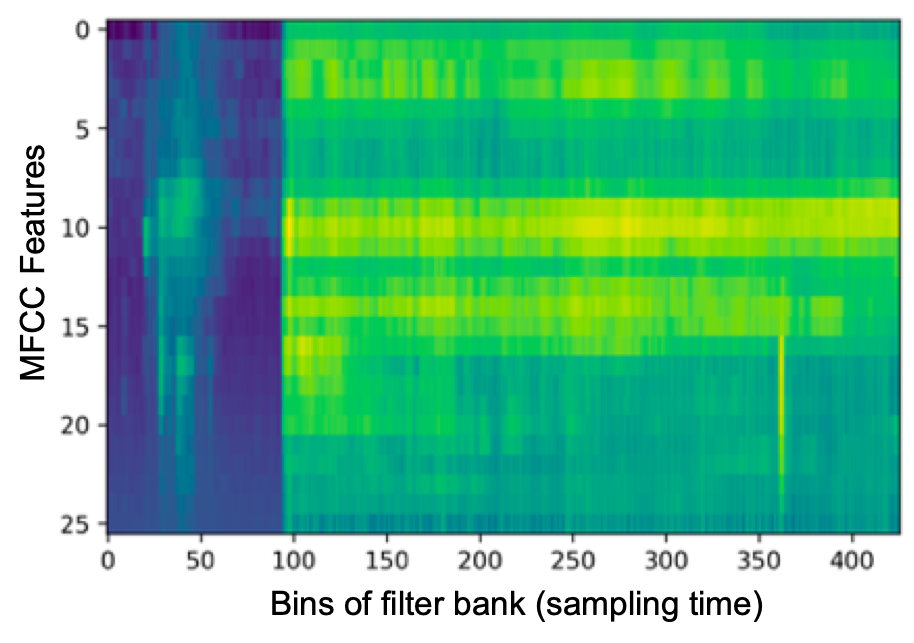
\includegraphics[width=0.4\textwidth]{./imgs/mfccFig3-new.png} % requires the graphicx package
    \caption{The audio matrix and extracted MFCC matrix}
    \label{fig:audio_matrix_mfcc}
\end{figure}

\section{Models \& Results}

\subsection{VAE}

The VAE model is variational autoencoder, which is a generative model and can be used to generate the images based on the image dataset \cite{doersch2016tutorial}. In the implemented VAE model, the dense layer is added to the model \cite{ji2020multi} and the keras in tensorflow 2.0 is used to perform the VAE model according to the keras document \cite{kerasVAE}. Following the building step for the VAE models \cite{mediumVAE} and the supervised VAE model \cite{linkedinVAE}, our VAE are built as the following architecture.

As is shown in Figure \ref{fig:vae_diagram}, there is one layer to load the pre-processed data into the model. In this data loader, the pre-process MFCC matrices are sliced by the sliding window with the sliding step of 96 frames. The input MFCC matrices are therefore in the dimension of $R^{96\times26}$. The following layer flattens the MFCC matrices as the dimension of $R^{48\times52}$ to load into the encoder and the decoder. The dimension of the latent is set to two, and the latent layer is transferred into the dense layer to predict the labels after being activated by the softmax function. The labels used in the VAE model are considered the type of the input audio files, such as the breath, the count, the vowel. Therefore, there are totally 18 labels for all the labels and the next step is to map the related 18 labels into binary classifiers as ‘COVID positive’ and ’COVID negative’.

\begin{figure}[htbp]{}
	\centering
    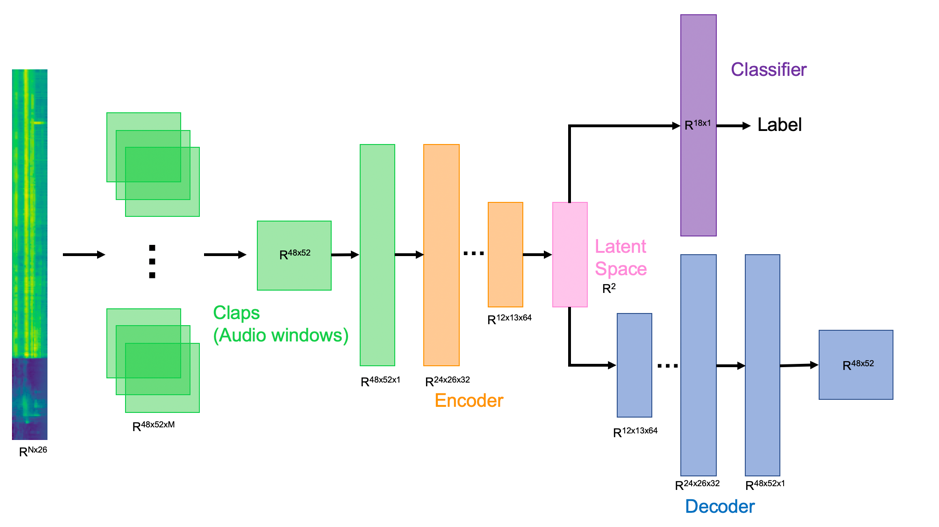
\includegraphics[width=0.8\textwidth]{./imgs/vaeDiagram.png} % requires the graphicx package
    \caption{The architecture of the VAE model}
    \label{fig:vae_diagram}
\end{figure}

In the training process, the loss function is defined as the combination of the kl-loss, reconstruction loss and clf-loss. By comparing with the possible combination of the loss function, the clf-loss is then defined as the main loss function for the training step in our COVID audio dataset. The train dataset and the test dataset is spliced by eighty percent of the data and the batch\_size is set to 128. The epochs are set to be 2 because the model will soon be optimized by the Adam optimizer and training too many times will lead to the exploding gradient problem according to our experiments to find the proper number of the epochs.
 
After training, the metrics are calculated by the sklearn packages in the testing dataset, which is previously spliced in the first layer of the VAE model. The ROC-AUC score, precision score, recall score, accuracy score, F1 score are calculated by the average of weight method. In the 18 labelled level, the ROC-AUC score of the VAE model is 0.8661, the precision score is 0.2366, the recall score is 0.3472, the accuracy score is 0.3472, and the F1 score is 0.2442.
 
When transferring the 18 labels mapped into the binary labels as ‘COVID-positive’ and ‘COVID-negative’, the ROC-AUC score of the VAE model is 0.5825, the precision score is 0.5685, the recall score is 0.6342, the accuracy score is 0.6342, and the F1 score is 0.4925. When checking the binary labels for the VAE model in the test dataset, it is surprising to find that even though there are differences in the eighteen labels, the binary labels are higher than eighteen labels as for the metrics among all the predicted labels in the test dataset. This shows that using the binary label to evaluate the VAE model is better than using the eighteen labels which is used in the training process. This also indicates that although the eighteen labels are different, the VAE model turns out to predict the patients as the positive patients and may be overfitted during the training process.

When drawing the latent space (Figure \ref{fig:latent_space}) for the test dataset in VAE model, it is evidently shown that when labelled with both audio types and the COVID-positive label, the latent space can be classified in different clusters or groups as shown in the left figure. However, if we use the binary label instead, different dataset will cluster together in this case, which is also the same as the metric performance as the above calculation.

\begin{figure}[htbp]{}
	\centering
    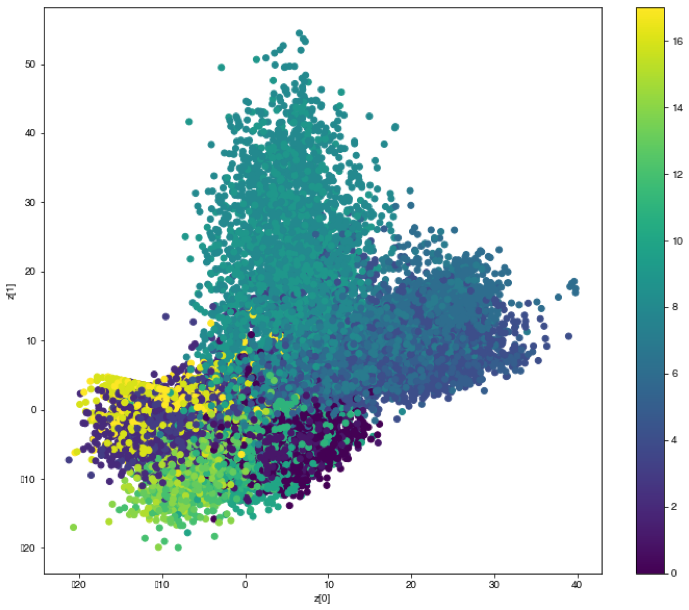
\includegraphics[width=0.4\textwidth]{./imgs/latentSpace1.png} % requires the graphicx package
    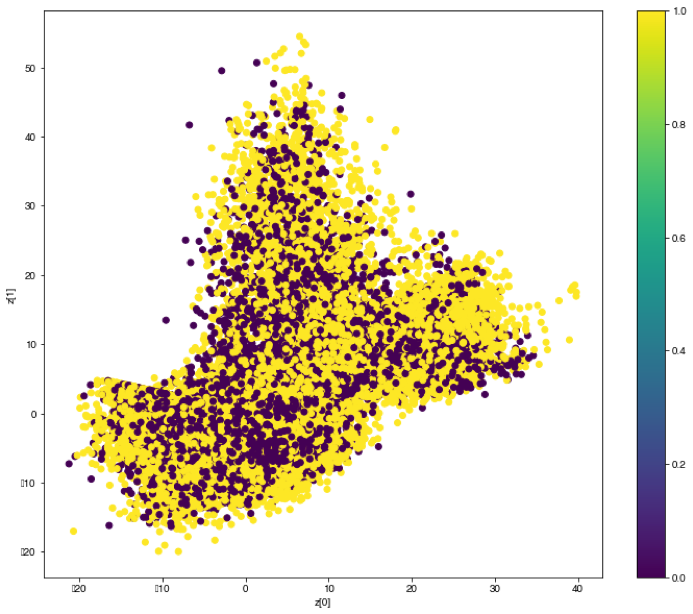
\includegraphics[width=0.4\textwidth]{./imgs/latentSpace2.png} % requires the graphicx package
    \caption{The visualization of the latent space in VAE model}
    \label{fig:latent_space}
\end{figure}

\subsection{GRU}

The GRU (Gated Recurrent Unit) was proposed by \cite{cho2014properties}, its structure was shown as follow in Figure \ref{fig:gru_structure}. It can make each recurrent unit adaptively capture dependencies of different time scales. The GRU has gating units that modulate the information flow inside the unit. However, it does not have any separate memory cells.

\begin{figure}[htbp]
	\centering
	\begin{minipage}[t]{0.48\textwidth}
		\centering
		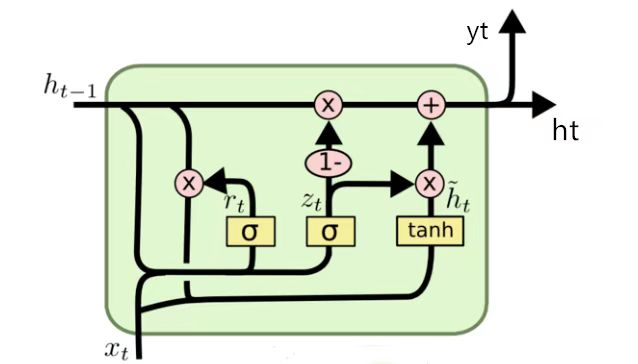
\includegraphics[width=1.0\textwidth]{./imgs/gru1.jpg}
		\caption{The structure of the GRU}
    	\label{fig:gru_structure}
	\end{minipage}
	\begin{minipage}[t]{0.48\textwidth}
		\centering
		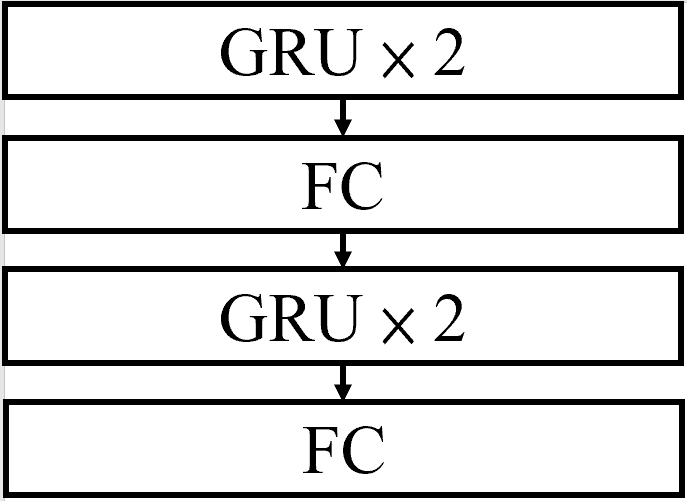
\includegraphics[width=0.6\textwidth]{./imgs/gru2.png}
		\caption{The structure of the implemented GRU based model}
    	\label{fig:implemented_gru_based_structure}
	\end{minipage}
\end{figure}

In the experiment, we chose to use the PyTorch platform to implement our model. For the preprocessing of the GRU model, when the voice data contains values that are less than -20, we consider this data as noise data and drop it. After this step, we obtained 559 patients’ valuable data.

Then we cut the data remaining into time stamps, and each time stamp contains 96 lines of data (which correspond to 960ms). After this step, we generated 4876 timestamps from the 559 patients, and later we would carry out classification tasks on each of the timestamps. Other than the 26 features extracted from the MFCC, we chose to add five features: Age, Gender, Location\_country, Location\_state, and English Proficiency as additional features to our input matrix; we use the hard encode method to encode these features. For the labels, at this part, we only consider two labels, which means if the patient is not healthy, it is label 1, otherwise label 0 (In total, we have 3581 label 0, and 1258 label 1).

We split the dataset into the training part (80\% of the original data) and the testing part (20\% of the original data) during the training stage. We also set the epoch number to 5 and the dropout rate of the GRU layers to 0.1 to prevent overfitting.

We use four GRU layers to encode the features and the time series. Firstly, use two GRU layers and a linear layer to encode the time stamp, then use another two GRU layers and a linear layer to encode the features; since the linear layer is the last layer of our model, we use its output to carry out the binary classification directly. The model structure is shown as follow in Figure \ref{fig:implemented_gru_based_structure}.

We chose the Adam optimizer with a learning rate equal to 0.001 and the Cross-Entropy loss function. Furthermore, we chose ten as our batch size. As a result, each forward process of our model has an input R, the shape of which would be (10, 96, 31). The result of the GRU model is shown in Table \ref{tab:cmp_model}. (Take four decimal places after the decimal point)

Although some of the metrics seem promising, the ROC-AUC score is only slightly over 0.5, which means this method still could not sufficiently capture the characteristics of the data. For future works, implementing some more complex models based on the GRU may solve this problem.

\subsection{LSTM}

CNN and RNN are the most commonly used model structures in deep learning. Most of the time, we will use CNN to process spatially structured data and RNN to process time series data. This time we need to deal with sound data, which is also a type of time series data. Here we try to use LSTM \cite{hochreiter1997lstm}, a classical RNN model, to capture the features in the data and see if we can accurately predict the health status from audio data.

The common model structure of LSTM is shown in Figure \ref{fig:lstm_structure}. It is a special type of RNN that invokes a gate mechanism for controlling the flow and loss of features, so that long-term dependency information can be learned.

\begin{figure}[htbp]
	\centering
	\begin{minipage}[t]{0.48\textwidth}
		\centering
		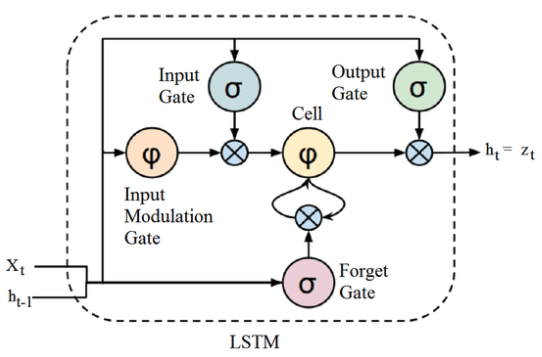
\includegraphics[width=1.0\textwidth]{./imgs/lstm.png}
		\caption{The structure of the LSTM}
    	\label{fig:lstm_structure}
	\end{minipage}
	\begin{minipage}[t]{0.48\textwidth}
		\centering
		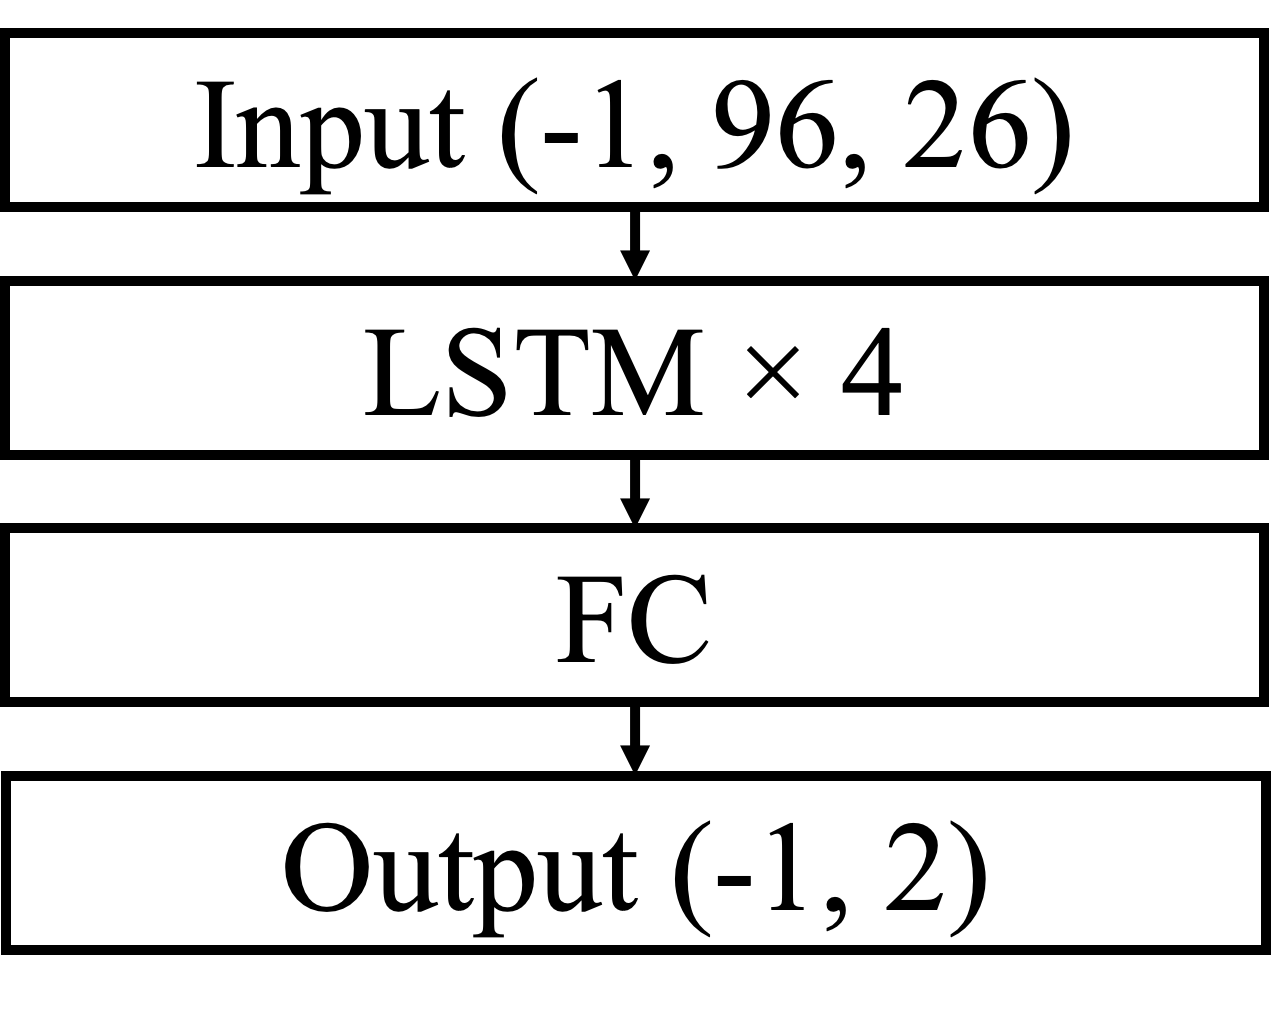
\includegraphics[width=0.6\textwidth]{./imgs/implemented_lstm.png}
		\caption{The structure of the implemented LSTM based model}
    	\label{fig:implemented_lstm_based_structure}
	\end{minipage}
\end{figure}

The commonly used deep learning frameworks are Tensorflow, PyTorch, etc. 
Here, we use PyTorch to complete the model part of the implementation, and 
make use of open source Python libraries such as scikit-learn and numpy to process and slice the data. 
The first dimension represents the number of time frames of the audio data, 
and the second dimension is the frequency bin. In the actual training process, 
we trim the audio data by truncating 96 consecutive frames from them to 
facilitate the training of the model and to avoid overfitting. 
Similar to the previous model, we treat the label with a healthy covid\_status as 1 and 
the rest as 0, which indicates a binary classification problem. 
In particular, we compress the data with pickle in order to avoid reading the file frequently 
during each training, and only need to process the data for the first time. 
We can easily load the processed data directly during training and debugging. 
For the selection of model hyperparameters, we tried various combinations and 
finally used 4 LSTM layers where each hidden layer has 64 dimensions (Figure \ref{fig:implemented_lstm_based_structure}).

To make the results easy to reproduce, we fixed random seeds from common libraries 
such as PyTorch, numpy, and random. To shorten the training time of the model, 
we trained the model on a NVIDIA GeForce RTx 2080 Ti GPU with a total of 200 epochs, 
which can be run in dozens of minutes. The initial learning rate was set to 0.001, 
and several experiments showed that setting a higher learning rate resulted 
in the model failing to converge. The batch size is 32, Adam optimizer is used to 
optimize the parameters and cross entropy is used to evaluate the loss of the model.

Compared to the complex models such as BERT \cite{devlin2018bert} and GPT \cite{floridi2020gpt} 
that are emerging in the field of natural language processing (NLP), the LSTM model is relatively simple, 
but at the same time has the advantage of not requiring a large amount of data for pre-training and 
the difficulty of simulating convergence is relatively low. The experimental results in 
Table \ref{tab:cmp_model} show that the LSTM model can achieve 0.7179 accuracy, 0.7342 precision, 
0.8871 recall, 0.8035 F1 score, and 0.6452 ROC-AUC score on Coswara dataset. 
The higher recall value indicates that the trained LSTM model is less likely to miss unhealthy samples.

\subsection{VGGish}

VGGish used in the classification task is performing a feature extraction job to produce embeddings from preprocessed audio inputs (MFCC) which will then be fed into another model for covid cough sound classification. 

VGGish feature extractor (Figure \ref{fig:vggish}) is established as a CNN model with a series of convolutional, activation, and max-pooling layers (17 layers in total). Publicly available pre-trained weights obtained by training the VGGish model on AudioSet are then loaded on the model created. 

\begin{figure}[htbp]{}
	\centering
    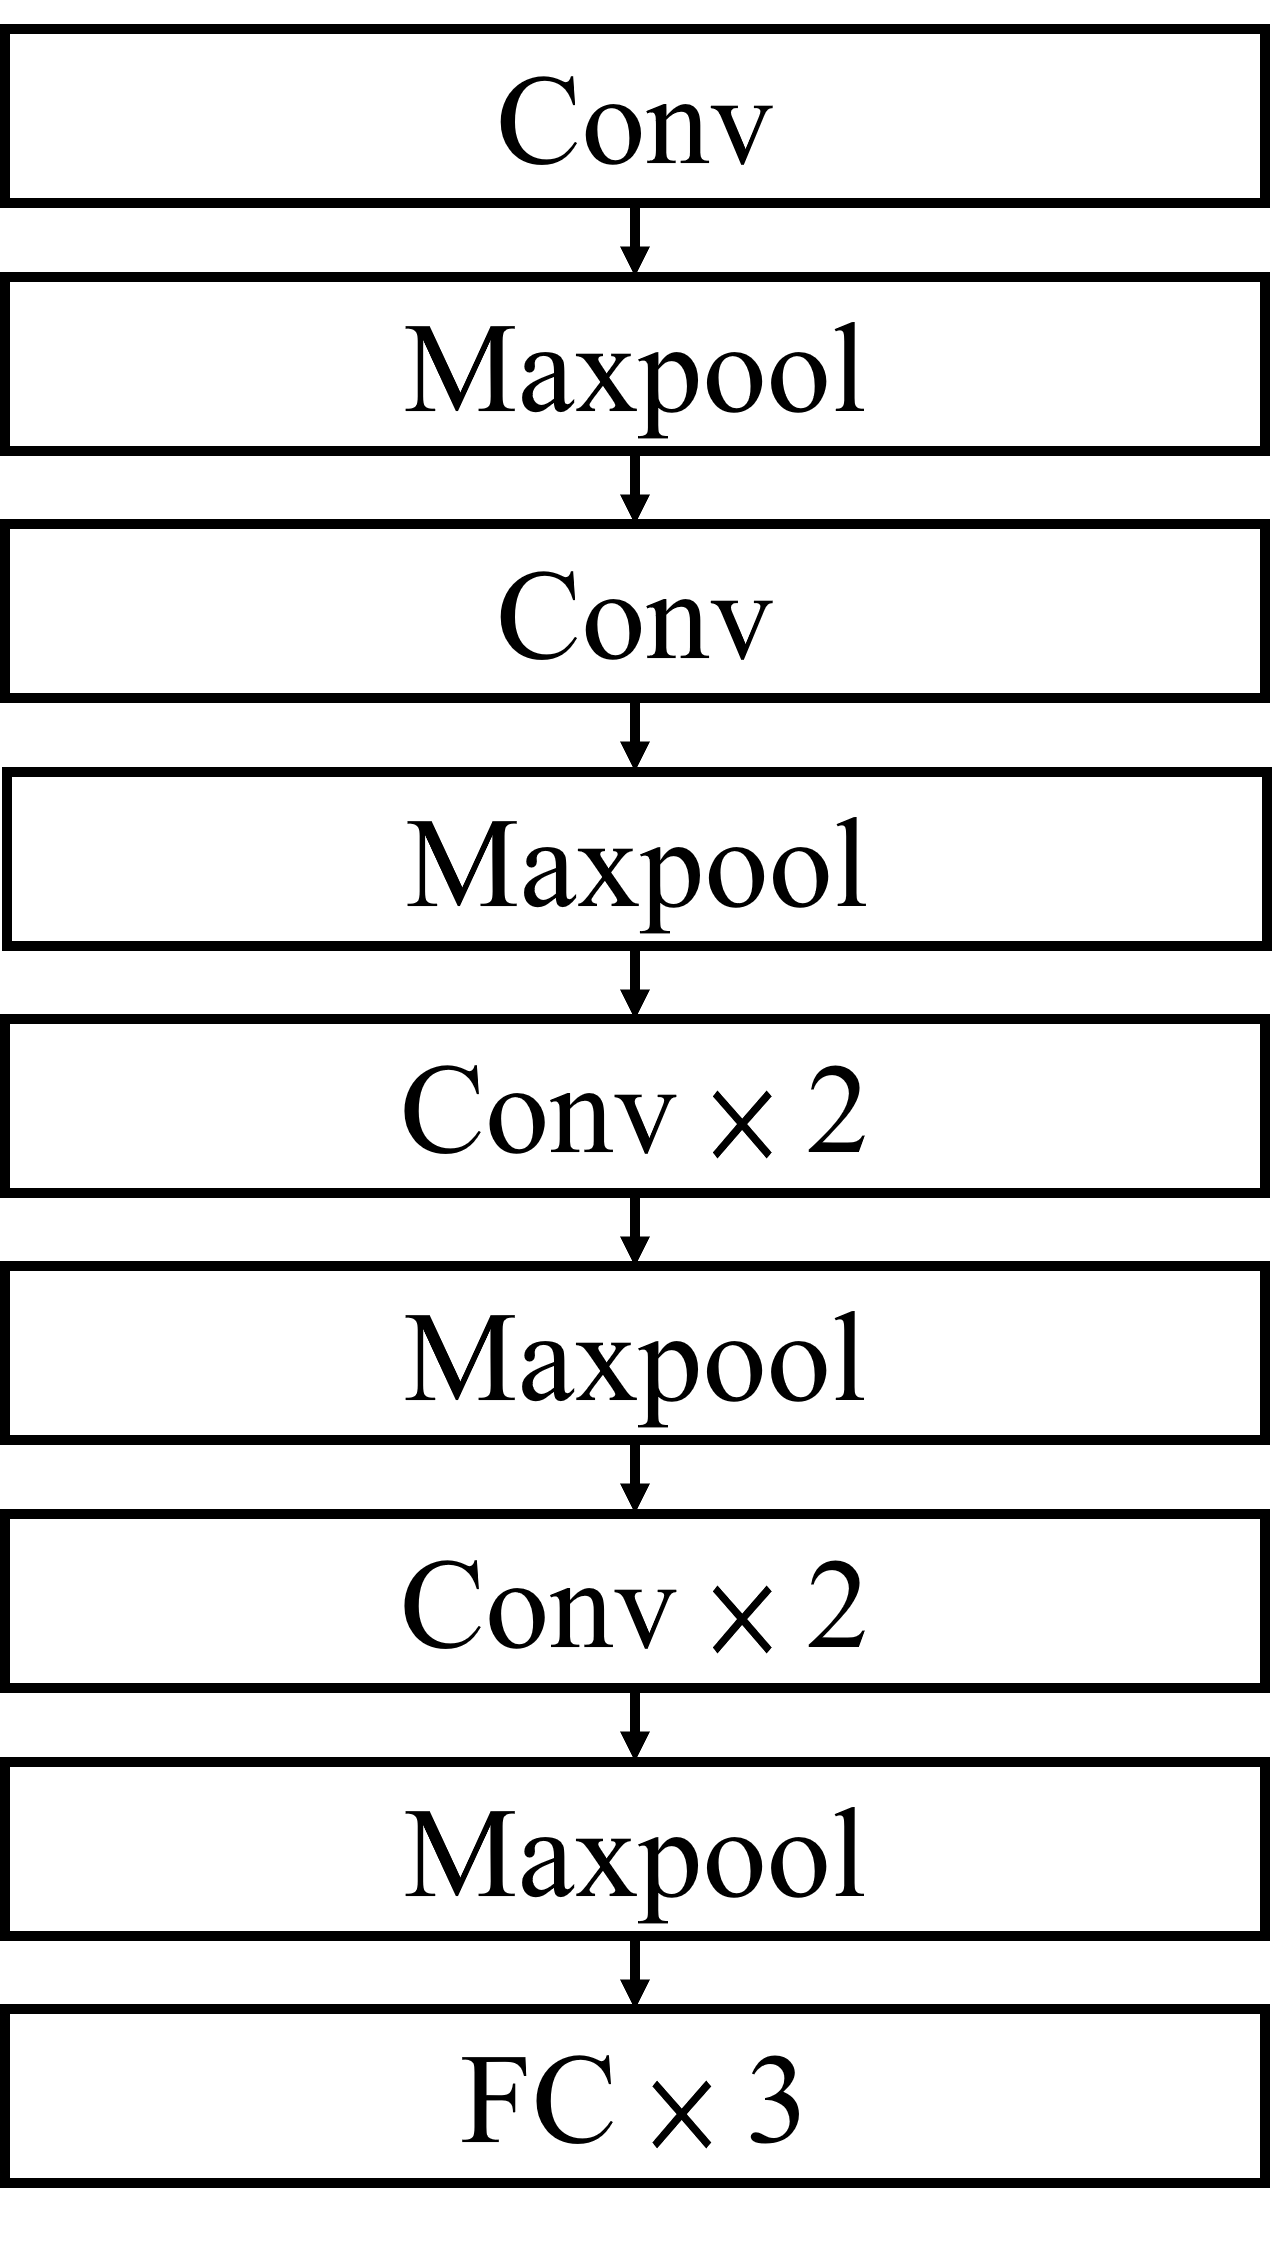
\includegraphics[width=0.2\textwidth]{./imgs/vggish.png} % requires the graphicx package
    \caption{The model structure of VGGish}
    \label{fig:vggish}
\end{figure}

The downstream model was constructed as a simple neural network with two convolutional layers and one activation layer with drop out adopted. The final output is activated by a sigmoid function for a binary classification task. This model would then take in the 128 D extracted feature and predict whether it is a healthy cough sound or a covid positive cough sound. 

During the training stage, input preprocessed audio data was splitted into training, validation and testing at a 0.8, 0.1, 0.1 ratio randomly with a batch size of 32. The loss function adopted in our experiment is BCE loss (Binary Cross Entropy loss) to measure the loss between a set of probabilities and a set of binary targets while the optimizer that follows is an Adam optimizer. Number of training epochs was set to 5 to prevent overfitting based on our experiment result. And the threshold to determine whether an example is healthy or covid positive is set to 0.5.

Trained with 1710 VGGish-extracted embeddings in total, the model can successfully perform the prediction task with a 0.8012 accuracy rate. Other metrics on the model including precision, recall, F1 score and ROC AUC score are 0.6419, 0.8012, 0.7127 and 0.5569 respectively. Though most metrics demonstrate pretty positive results, the ROC AUC score is slightly lower than what was expected. After taking a deeper look at the input data itself, a problem of imbalanced data was discovered. Thus the slightly higher than 0.5 ROC AUC score means that the model can not separate the two classes very well. It is highly likely that the model predicts most examples as healthy as there are more healthy examples in the data intrinsically.

To improve on that, oversampling on the minority class was performed. The number of covid positive samples was increased to 1287 by random oversampling to match the number of healthy examples. With a balanced input dataset, most training conditions were set to be the same as the previous imbalanced data experiment while the learning rate of the Adam optimizer and the number of epochs were set to a greater number, which is 0.005 and 100 respectively. 

The newly trained model gives a result of 0.7519 accuracy rate and 0.7636, 0.7519, 0.7485, and 0.8095 for precision, recall, F1 score, and ROC AUC score respectively. While the accuracy rate and the precision is moderately lower than the training results from imbalanced input data, all the other metrics are benefited from training with a balanced set of data. As the ROC AUC score is significantly higher than the previous result, we know that the model is now more capable of distinguishing the two classes. 

The results obtained here (Table \ref{tab:cmp_vggish}) are more similar to the ones presented in the paper we selected. The possible reason why recall is higher than what was presented in the paper might be that we had more original examples of healthy cough sounds (labeled 1) so that the model can actually learn better on this particular label. Other metrics being moderately lower might be stemming from the fact that we haven’t fine tuned the parameters enough and we are using repeating covid positive cough sounds to train the model. 

\begin{table}
	\centering
	\begin{tabular}[!htbp]{|c|c|c|c|c|c|}
	\hline
	& Accuracy & Precision & Recall & F1 Score & ROC-AUC\\
	\hline
	Experiment results with imbalanced data & 0.8012 & 0.6419 & \textbf{0.8012} & 0.7127 & 0.5569\\
	\hline
	Experiment results with balanced data & 0.7519 & 0.7636 & 0.7519 & 0.7485 & 0.8095\\
	\hline
	Results in the paper (without fine-tuning) & 0.8071 & 0.7855 & 0.6742 & 0.7256 & 0.8502\\
	\hline
	Results in the paper (with fine-tuning) & \textbf{0.8312} & \textbf{0.8315} & 0.6949 & \textbf{0.7571} & \textbf{0.8734}\\
	\hline
	\end{tabular}
	\caption{Comparison between experiment results and paper implementation results}
	\label{tab:cmp_vggish}
\end{table}

\subsection{Transformer-AST}

Transformer is proposed in 2017 and appies the attention layer for data processing. A fully supervised method relies heavily on the annotation. However, high quality annotation of the COVID-19 sound data is not fully available, which renders a challenge for the supervised based method for COVID-19 classification. The purpose of the transformer model is to train a feature encoder to learn from a large amount of unlabeled sounds. However, due to the high computation demand and time consuming for the Transformer-CP model, we choose to implement the Transformer-AST (audio spectrogram transformer) model as proposed by Yuan Gong (Figure \ref{fig:transformer_ast}) \cite{gong2021psla}.  

\begin{figure}[htbp]{}
	\centering
    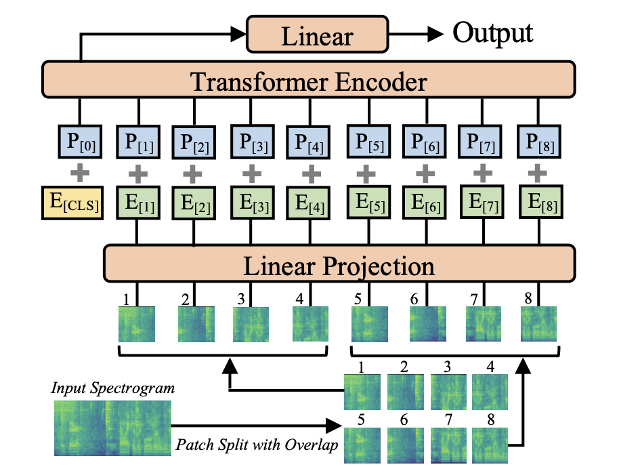
\includegraphics[width=0.8\textwidth]{./imgs/transformer_ast.png} % requires the graphicx package
    \caption{The proposed audio spectrogram transformer (AST) architecture \cite{gong2021psla}}
    \label{fig:transformer_ast}
\end{figure}

In the Transformer-AST model, the cough sound tracks of 2063 participants in the wav format were included for analysis. We first computed the mean and standard deviation of the sound dataset for downstream normalization. Secondly, the dataset was splitted into 5 folds for training and evaluation. For both the frequency and the time dimension, we splitted with a stride of 10. Neither ImageNet nor AudioSet pretrained model was included because inclusion of them took longer time and did not help achieve better improvement, just made the result almost like a random classification. Totally 5 epochs and a learning rate of 1e-4 were used for training. Adam optimizer and cross-entropy loss were selected in this model.

Transformer-AST is a convolution-free model and contains just the self-attention architecture. Spectrogram masking was applied for both time and frequency dimension, with the former set to 24 and the latter set to 96. With masking, we tried to avoid overfitting problems. This model achieved high performance as mentioned in the original paper, but its performance was limited when applied to COVID-19 sound dataset. The AUC is only 0.5825. Although different scenarios like the epoch number and data normalization were also tried, there is no better achievement. Further investigation of the architecture of the transformer might help illustrate such problems.

\section{Comparison of the models}

Table \ref{tab:cmp_model} shows the result of the five models introduced in the paper. The VGGish model produced the best result, with the ROC-AUC score equal to 0.8095. For other models, although some of them may have a higher Precision score or Recall score. Their ability to distinguish between classes is not comparable with the VGGish model.

\begin{table}
	\centering
	\begin{tabular}[!htbp]{|c|c|c|c|c|c|}
	\hline
	Model & Accuracy & Precision & Recall & F1 Score & ROC-AUC\\
	\hline
	VAE & 0.6342 & 0.5685 & 0.6342 & 0.4925 & 0.5825\\
	\hline
	GRU & 0.7349 & \textbf{0.9919} & 0.7391 & \textbf{0.8470} & 0.5257\\
	\hline
	LSTM & 0.7179 & 0.7342 & \textbf{0.8871} & 0.8035 & 0.6452\\
	\hline
	VGGish & \textbf{0.7519} & 0.7636 & 0.7519 & 0.7485 & \textbf{0.8095}\\
	\hline
	Transformer-AST & 0.6457 & 0.5054 & 0.0692 & 0.1217 & 0.5825\\
	\hline
	\end{tabular}
	\caption{Result of the five models introduced in the paper}
	\label{tab:cmp_model}
\end{table}

\section{Conclusion}

\paragraph{The binary labels and extracted MFCC features contributes to the classification of each model.} According to the meta information together with the COVID testing label, we found that applying the binary label (healthy label which is COVID negative and unhealthy label which is COVID positive) matters in the classification of the patient audios. The extracted MFCC matrices and all the implemented models can perform the classification of the patient audio and make the prediction for the COVID testing status or the healthy status with the COVID labels. Among different models, the comparison is made and the results are drawn as subsequent conclusions.

\paragraph{LSTM is the best model to classify the patient audios.} From the above results, LSTM is the best model to classify the healthy condition based on the audio of patients regarding the precision score. The LSTM model has the highest recall score, indicating that the model will predict less false negative results than other models and retrieves the healthy label for the patient audios. As for the COVID detection level, the LSTM model will tend to classify the patient audios as the healthy, which is COVID negative.

\paragraph{GRU is the best model to make decisions on COVID testing.} Nevertheless, suppose we are making a conservative testing for the patient's audio, we should choose the model with high precision and low recall. Indicating that the model will be likely to classify the patients as the unhealthy which is COVID positive and the patients will be followed up with further detection in this case. Notwithstanding that the VAE model and the Transformer-AST model have the lower recall score, these two models have too low precision score and are likely to recognize the patient audio as COVID-positive (unhealthy label) mostly, which is not appropriate to the decisions determined by the classification model. Such a model is truly the GRU model and it will be conservative to make the decision on whether the patient is healthy or not along with higher precision on classification of the COVID patient audios. 

\paragraph{Suggestions on diagnosis methods}
Proceeded from previous results among various models we implemented, it is achievable to manipulate the audio information to classify the COVID positive and COVID negative patients, for example the audios from the breath, cough, counting and vowels, which can be the application to the detection and the diagnosis to the COVID or the healthy condition for the patients. With respect to the preference of the classification models, it is suggested to use the strictly negative model to diagnose in the occasion of the final decision or the high throughout occasion and utilize the negative friendly model combined with other COVID testing method so as to avoid the false negative testing outcomes for COVID-positive patients.


\section{Future Work}

The future work lies on three aspects, incoming audio data, training of the models and the requisition in COVID diagnosis. 
For the incoming audio data in the future, our dataset needs to update due to the increasing number of the COVID patient audio. In this circumstance, the best models for diverse occasions should also be trained with the updated dataset in which process will occupy most of the time and space. Besides, the models and the training process could also be refined in the future. Eventually, since currently the model is in theory, the trained model will be applied to the diagnosis in COVID-19 in the future.

\section{Contributions}

The team members are in equal contributions.

\paragraph{Chung-chi CHAO}

My contribution to the project is focused on the experiments on VGGish,
the final report section on VGGish and the related work section in the final report. 
I have researched on the VGGish model and try to replicate the experiments done 
in our selected paper using the publicly available pretrained weights mentioned in the paper. 
After identifying the problem of imbalanced data, I have also attempted to solve the problem by oversampling. 
Afterwards, I repeated the experiment and tried to fine tune the parameters. 
Following that, I summarized my experiment results in the final report. 
In the end, I put together related work which is doing a similar COVID-19 classification 
task in the related work section in the final report.

\paragraph{Jiabao LI}

My contributions in the group project consist of the data pre-process and the Variational 
Autoencoders model (VAE model) part. In the data pre-process part, I extracted the audio 
files for all the patients and then cleaned the audio files to make sure that 
all the patients had the available audio files. The digital signal processing methods 
were exploited to extract the mel frequency cepstral coefficients (MFCC) matrix for the audios 
of all the cleaned patients with the log-compressed filter tank. In the VAE part, 
I implemented the VAE model to train our data based on the reference article, 
after which the metrics were calculated focusing on the test dataset which was twenty 
percent of the whole input extracted MFCC dataset. Ultimately, I wrote the conclusion part 
with reference to the repercussions in our implementation.

\paragraph{Zongchao MO}

My contribution is to implement the Transformer-AST model. In this part, 
I use the cough sound track dataset to train a transformer model and predict 
whether a participant is COVID-19 positive. In building this model, I tried different 
models that took different formats of data as input. Afterwards, I wrote the corresponding 
result part of this model in this report and integrated the background section for this 
report based on the previous proposal. And also, I searched across various topics and 
articles and recommended this one for my groupmate at the beginning. 

\paragraph{Jihong TANG}

For this course project in COMP5331, my work contribution could be divided into two parts: 
data analysis work and paperwork. For the data analysis work, I focused on the 
analysis of raw data from coswara project. Descriptive analysis and correlation analysis 
of the 2128 subjects are done to reveal that the binary labeling system is useful in our project. 
For the paperwork, I firstly drafted and combined the project proposal based on the revised 
Latex template I provided for the whole project. Secondly, I wrote all the related analysis 
work in the final report and made the final recheck before the submission of the report. 
Thirdly, I combined all the materials and designed them to become our final project presentation slides. 

\paragraph{Yubo WANG}

My contributions in the group project consist of the Gated Recurrent Unit (GRU) model part 
and the result comparison part. At the GRU part, I built up a GRU-based model and carried out 
a binary classification (to predict whether a patient has COVID or not) task using the coward dataset. 
I tried several model structures and chose the best one for the task. 
Based on the experiment result, I wrote the GRU model part. As for the comparison part, 
I compared all the five models implemented in this paper and carried out an analysis, 
find out the VGGish model was the best.

\paragraph{Lingyun YANG}

In this project, I was responsible for the implementation of the LSTM model and 
its application to the coswara dataset for classification and prediction of audio data. 
I also helped to provide a deeper understanding of the existing coswara dataset 
through an in-depth reading of the references to effectively carry out model construction 
and indicator evaluation. By continuously testing the structure and hyperparameters of the model, 
a relatively good performing LSTM model was trained. In addition, I was responsible 
for the integration and review of the project report, handling the citation format, 
and finally presenting everyone's results in LaTex form.

\newpage
\bibliography{KDD}
\end{document}
